\documentclass[aspectratio=169]{beamer}
\usetheme{Warsaw}
\usepackage{tikz}

\begin{document}
	
	\begin{frame}{Monatsübersicht}
		\framesubtitle{Tag für Tag}
		
		\begin{center}
			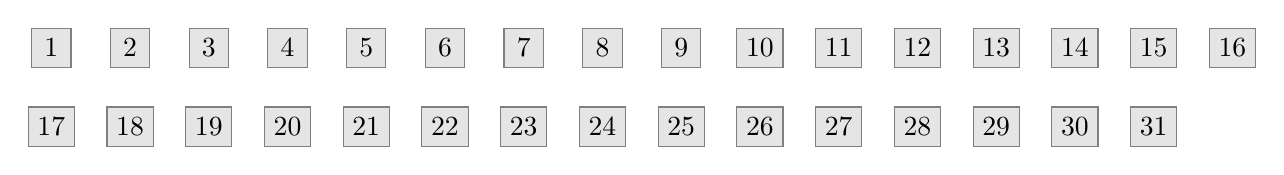
\begin{tikzpicture}
				% Einstellungen für die Kästchen
				\tikzset{box/.style={
						draw=gray, % Graue Linie für die Umrandung
						fill=gray!20, % Leicht graue Füllung
						minimum size=0.5cm, % Minimale Größe der Kästchen
						text=black, % Textfarbe
						align=center % Text zentrieren
				}}
				
				% 31 Kästchen erzeugen
				\foreach \n in {1,...,31} {
					% Kästchen positionieren
					\pgfmathtruncatemacro{\row}{(\n - 1) / 16} % Neue Zeile alle 16 Kästchen
					\pgfmathtruncatemacro{\col}{mod(\n - 1, 16)} % Spaltenposition berechnen
					\node[box] at (\col, -\row) {\n}; % Kästchen mit Nummerierung platzieren
				}
			\end{tikzpicture}
		\end{center}
		
	\end{frame}
	
\end{document}
